\subsection{Example: Inverted slider-crank Mechanism}

\begin{frame}
	\begin{block}{Example 3: Inverted slider-crank Mechanism}
		\begin{table}
			\begin{minipage}{0.5\linewidth}
				\begin{tabular}{l|l}
					      & $l_{AD}=l_1=0.35m$\\
					Given & $l_{BC}=l_2=0.20m$\\
					      & $l_{AC}=0.15m$\\
					      & $\theta_1=60^{\circ}$\\\hline
					Find  & $\vb{r}{B}$, $\vb{r}{D}$
				\end{tabular}
			\end{minipage}\hfill
				\begin{minipage}{0.5\linewidth}
					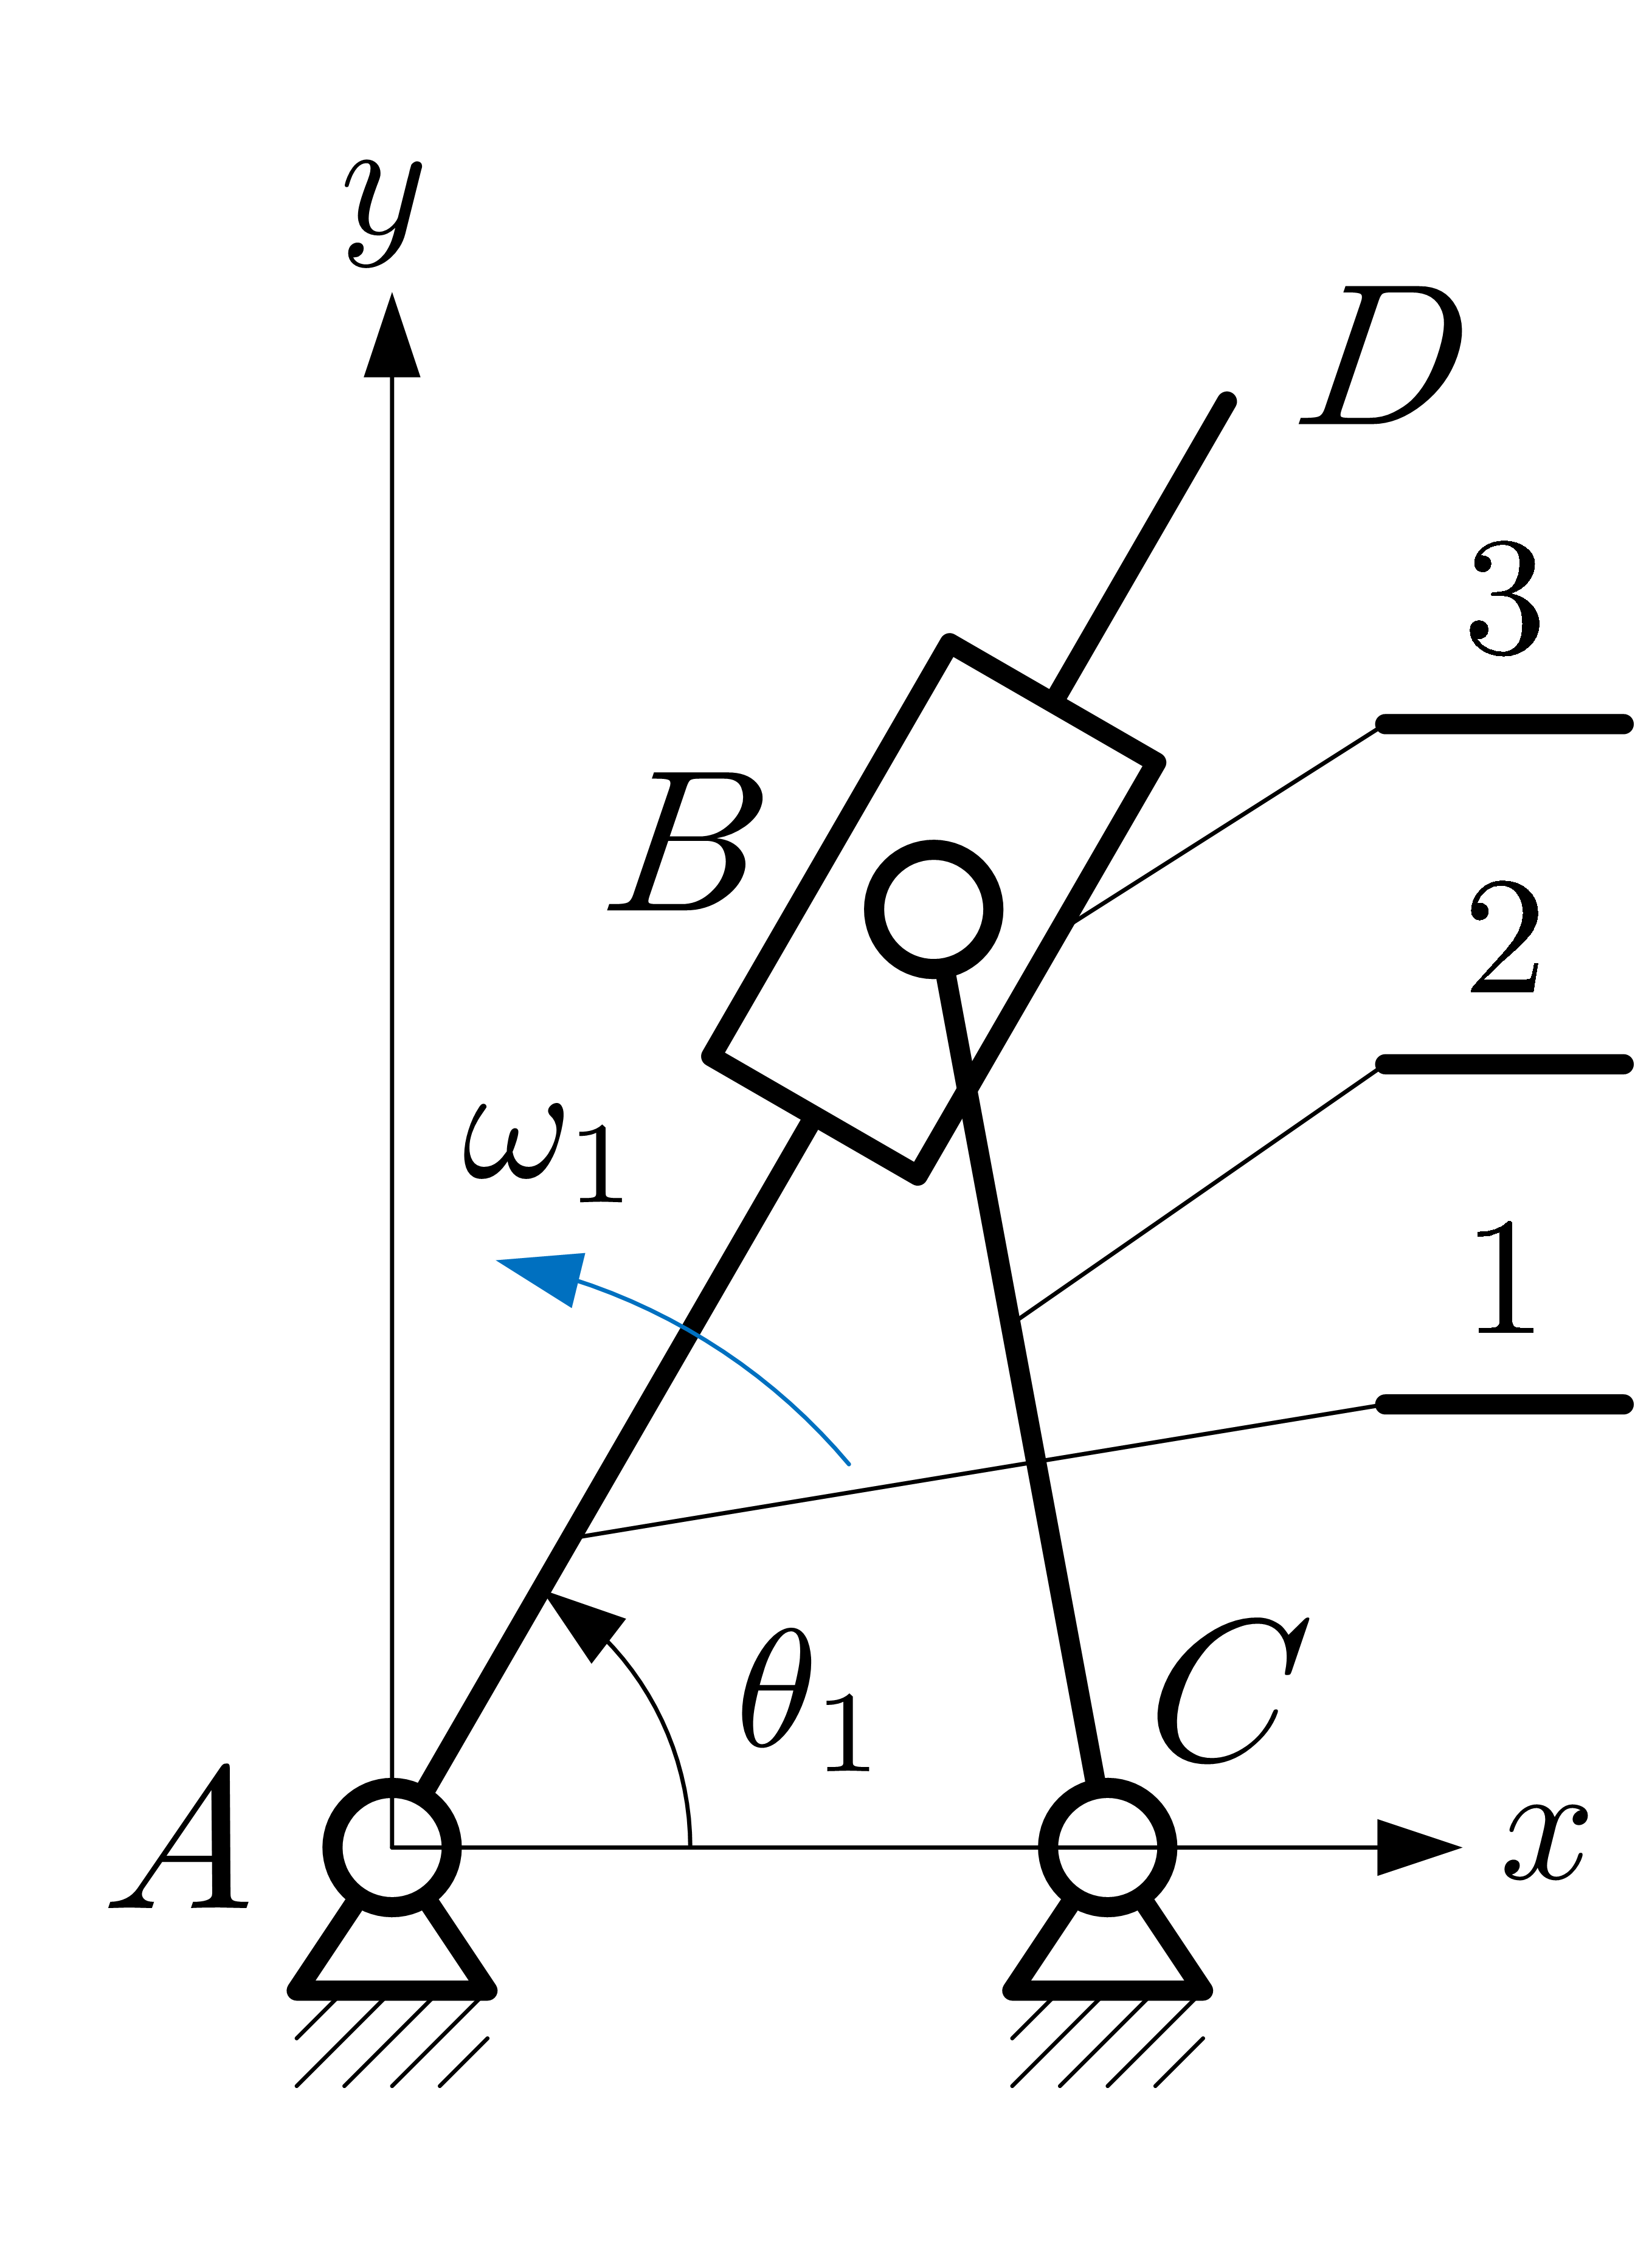
\includegraphics[width=30mm]{images/Inverted-R-RRT.png}
				\end{minipage}
		\end{table}
	\end{block}
\emph{Solution}\vskip2.5mm
Position of joint $B$: $\displaystyle \vb{r}{B} = x_B\ih + y_B\jh = l_{AB}\cos{\theta_1}\ih + l_{AB}\sin{\theta_1}\jh$\\
Position of joint $C$: $\displaystyle \vb{r}{C} = x_C\ih + y_C\jh = 0.15\ih$\\
Position of joint $D$: $\displaystyle \vb{r}{D} = x_D\ih + y_D\jh = l_1\cos{\theta_1}\ih + l_1\sin{\theta_1}\jh$
\end{frame}

\begin{frame}
\emph{Solution}\vskip2.5mm
Position of joint $B$: $\displaystyle \vb{r}{B} = x_B\ih + y_B\jh = l_{AB}\cos{\theta_1}\ih + l_{AB}\sin{\theta_1}\jh$\\
Position of joint $C$: $\displaystyle \vb{r}{C} = x_C\ih + y_C\jh = 0.15\ih$\\
Position of joint $D$: $\displaystyle \vb{r}{D} = x_D\ih + y_D\jh = l_1\cos{\theta_1}\ih+l_1\sin{\theta_1}\jh$
\[
\Rightarrow\displaystyle(x_B-x_C)^2+y_B^2=l_2^2
\]
\[
\text{ or } (l_{AB}\cos{60^\circ}-0.15)^2+l_{AB}\sin{60^\circ}=l_2^2
\]
Solving the system of equations yields $l_{AB}>0$ and $l_{AB}<0$. Then, choose $l_{AB}>0$ and substitute the result into $\vb{r}{B}$
\end{frame}


\begin{frame}{MATLAB R2019a code}
\lstinputlisting[style=Matlab-editor, basicstyle=\mlttfamily]{codes/Inverted-RRRT-position.m}
\end{frame}
\begin{frame}{Plotting using MATLAB R2019a}
\lstinputlisting[style=Matlab-editor, basicstyle=\mlttfamily]{codes/Inverted-RRRT-plot.m}
\end{frame}
\begin{frame}{Output figure}
\centering
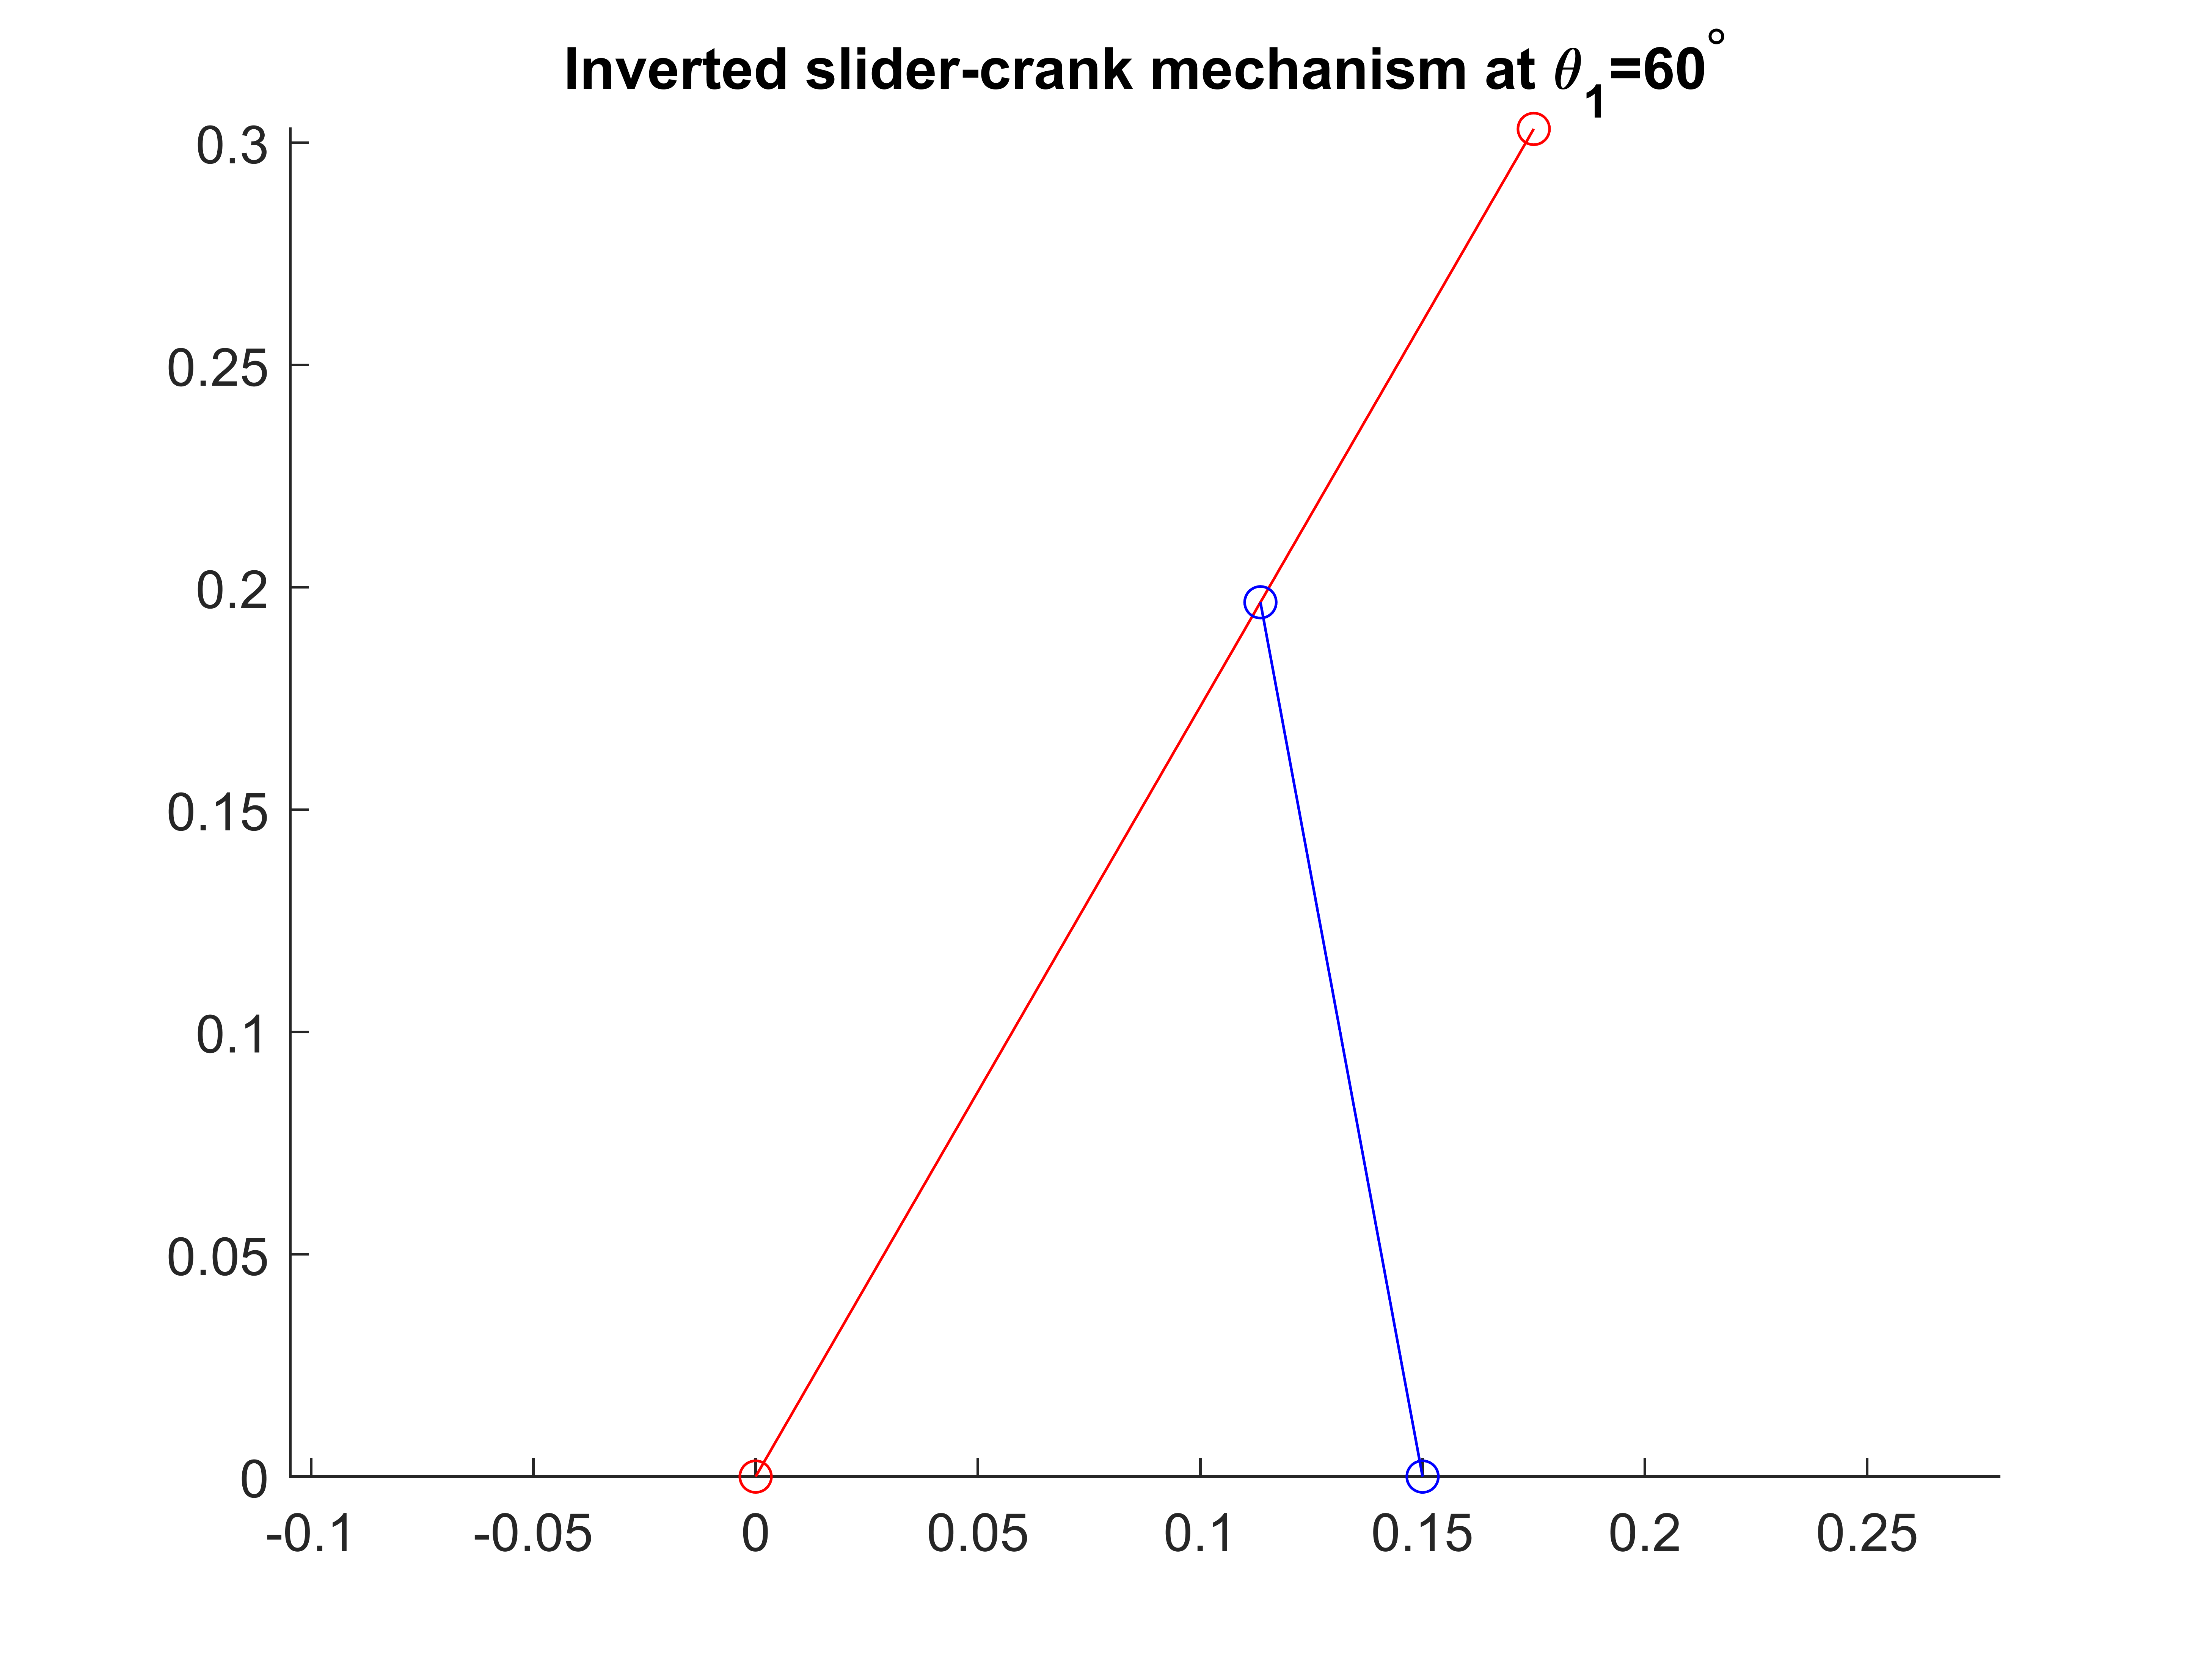
\includegraphics[width=100mm]{images/Inverted-RRRT-plot.png}
\end{frame}
\begin{frame}{Trajectory plotting using MATLAB R2019a}
\lstinputlisting[style=Matlab-editor, basicstyle=\mlttfamily]{codes/Inverted-RRRT-trajectory.m}
\end{frame}
\begin{frame}{Output figure}
\centering
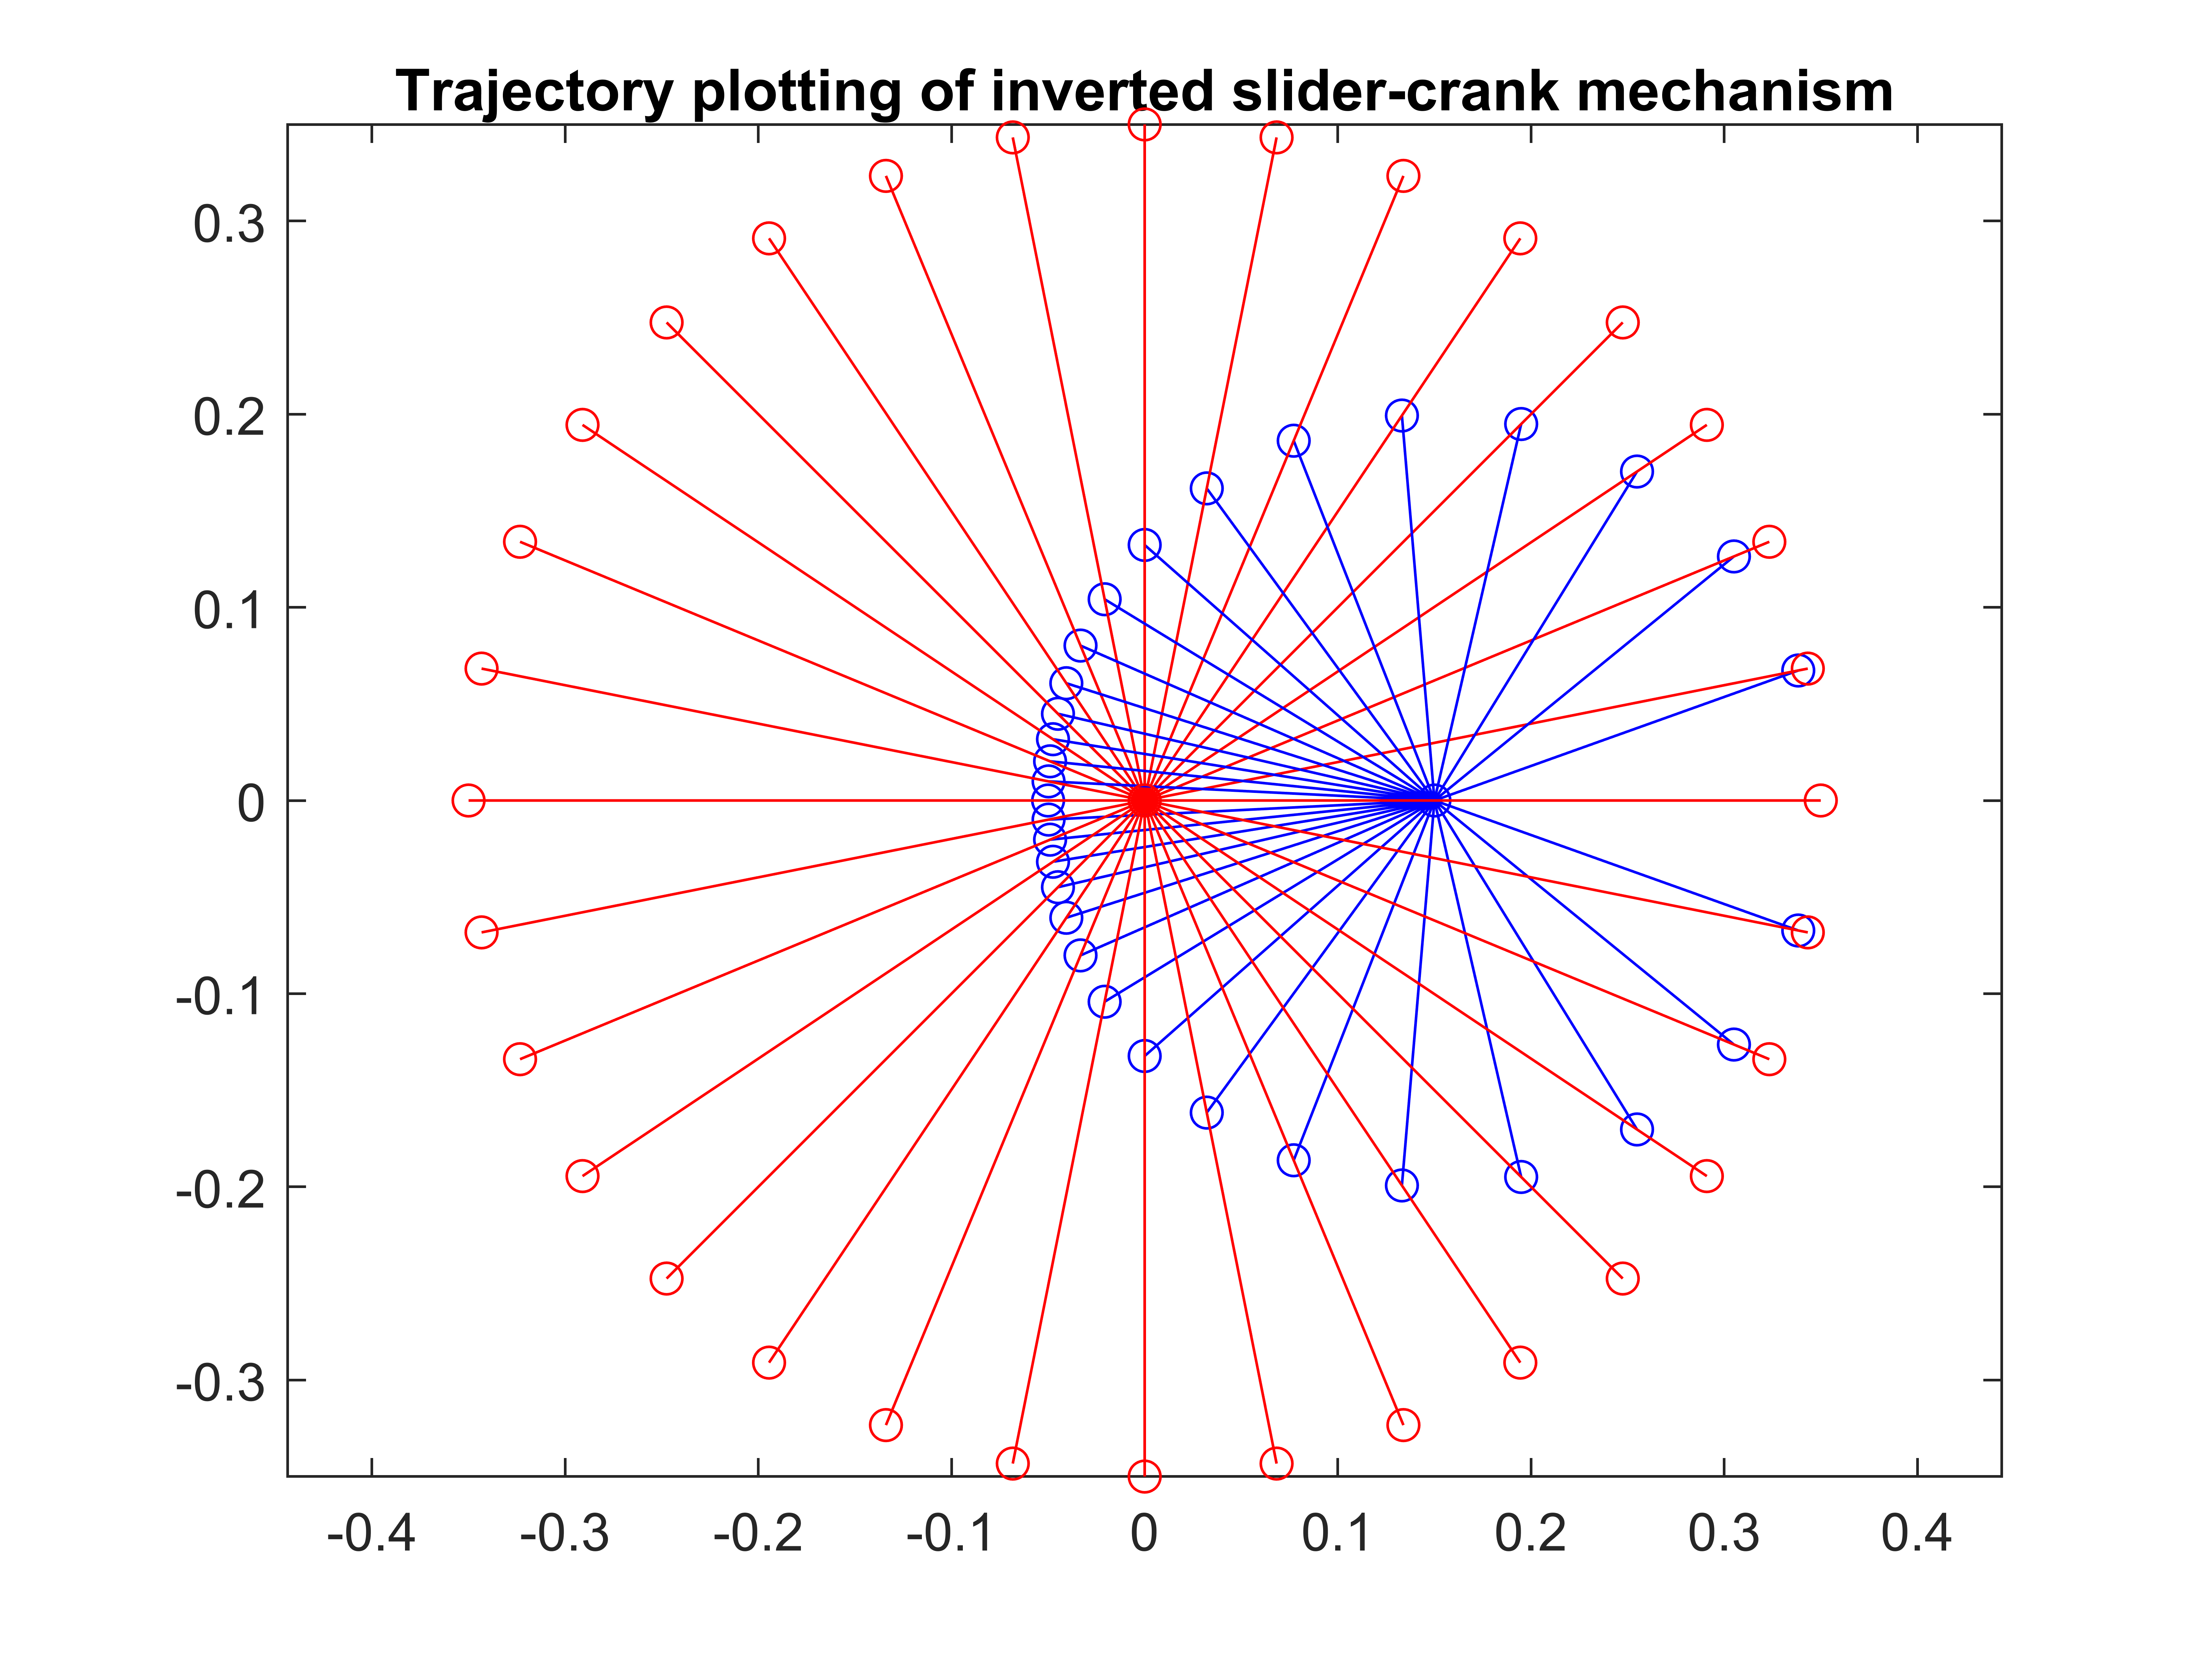
\includegraphics[width=100mm]{images/Inverted-RRRT-trajectory.png}
\end{frame}
